\documentclass[12pt]{article}

\usepackage{sbc-template}
\usepackage[utf8]{inputenc}
\usepackage[T1]{fontenc}
\IfFileExists{brazil.ldf}{\usepackage[brazil]{babel}}{}
\usepackage{graphicx}
\usepackage{amsmath}
\usepackage{url}
\usepackage{booktabs}
\usepackage{microtype}
\usepackage[htt]{hyphenat}
\setlength{\emergencystretch}{2em}

\sloppy

\title{Autoescalamento horizontal de Pods em Kubernetes: \\
       análise comparativa entre cluster local e cluster gerenciado}

\author{Ricardo Kenzo Akaki Ito\inst{1}}

\address{Escola Politécnica -- Universidade de São Paulo (USP)\\
  PSI5120 -- Tópicos em Computação em Nuvem
  \email{rkai03@usp.br}
}

\begin{document}

\maketitle

\begin{abstract}
This work evaluates the behavior of the Kubernetes Horizontal Pod Autoscaler
(HPA) in two distinct environments, a local Minikube cluster and a managed
Amazon EKS cluster. The same container image, the same manifests and the same
load profile were applied to both, so that observed differences could be
attributed to the infrastructure rather than to the artifact. Instrumentation
sampled the autoscaler state every five seconds and recorded a time series,
which allowed reaction time to be measured rather than merely observed. Results
show nearly identical detection latency, 16 and 14 seconds, and a twofold
difference in the time required to reach the replica ceiling, 74 seconds
locally against 35 seconds in the managed cluster.
\end{abstract}

\begin{resumo}
Este trabalho avalia o comportamento do Horizontal Pod Autoscaler (HPA) do
Kubernetes em dois ambientes distintos, um cluster local em Minikube e um
cluster gerenciado em Amazon EKS. Foram utilizadas as mesmas imagens de contêiner, os mesmos
manifestos e o mesmo perfil de carga foram aplicados aos dois, de modo que as
diferenças observadas pudessem ser atribuídas à infraestrutura e não ao
artefato executado. A instrumentação amostrou o estado do autoescalador a cada
cinco segundos e registrou uma série temporal. Os resultados mostram latência de detecção
praticamente idêntica, de 16 e 14 segundos, e diferença de duas vezes no tempo
necessário para atingir o teto de réplicas, 74 segundos no ambiente local
contra 35 segundos no gerenciado.
\end{resumo}

\section{Introdução}

A elasticidade é uma característica definidora da
computação em nuvem, entendida como a capacidade de ajustar recursos à demanda
sem intervenção manual.

O HPA opera segundo o modelo de reconciliação que caracteriza o Kubernetes. O
operador declara um estado desejado, expresso como faixa de réplicas e alvo de
utilização, e um controlador compara continuamente esse estado com o observado,
agindo quando divergem. A cada ciclo, cujo intervalo padrão é de quinze
segundos, o controlador consulta a métrica de utilização e calcula o número de
réplicas necessário segundo a expressão
\[
r_{\text{desejadas}} = \left\lceil r_{\text{atuais}} \times
\frac{u_{\text{atual}}}{u_{\text{alvo}}} \right\rceil
\]
onde $u$ representa a utilização média das réplicas.
 
A utilização não é medida em valor absoluto, e sim como proporção do recurso
declarado em \texttt{requests.cpu} no manifesto do contêiner. Se esse campo não
estiver definido, não existe denominador, o controlador não consegue computar a
métrica e o autoescalamento não ocorre, situação que se manifesta pela
permanência indefinida do valor \texttt{<unknown>} na saída de consulta do
objeto.

Este trabalho investiga se e como o comportamento desse controlador difere
entre um cluster local, executado em estação de trabalho, e um cluster
gerenciado em provedor de nuvem. A pergunta é pertinente porque o
desenvolvimento e a validação de aplicações frequentemente ocorrem em ambiente
local, ao passo que a operação ocorre em nuvem, e diferenças de comportamento
entre os dois afetam a confiança que se pode depositar nos testes locais.

A contribuição principal está no método. Em vez de constatar que o
autoescalamento ocorreu, a prática foi instrumentada para registrar uma série
temporal do estado do controlador, o que permite expressar o tempo de reação
como grandeza numérica e compará-lo entre ambientes.

\section{Arquitetura e topologia}

\subsection{Aplicação}

A carga de trabalho é um servidor web escrito em Python, sem dependências
externas, que expõe três pontos de acesso. Dois deles respondem imediatamente e
servem de alvo às sondas de saúde do Kubernetes. O terceiro, denominado
\texttt{/work}, consome processador de forma deliberada e controlada.

A carga é especificada por \emph{tempo de processador} e não por número de iterações. Se
fosse definida por iterações, um processador mais rápido concluiria o trabalho
em menos tempo e consumiria menos CPU-segundos por requisição. 

A precisão do mecanismo foi verificada antes da publicação da imagem. Para um
alvo de 200 milissegundos, o tempo efetivamente consumido foi de 200,34
milissegundos.

\subsection{Empacotamento}

A aplicação foi empacotada em imagem de contêiner a partir de \texttt{python:3.12-slim},
com usuário sem privilégios de identificador 10001 e execução sob a diretiva
\texttt{USER}, verificada após a construção. A imagem foi publicada em registro
público com a etiqueta \texttt{v1}, deliberadamente imutável, e o digest
resultante foi registrado. Uma etiqueta mutável como \texttt{latest} permitiria
que os dois clusters executassem conteúdos distintos sem aviso, o que
invalidaria a premissa central da comparação.

\subsection{Objetos declarados}

Cinco manifestos foram aplicados sem alteração nos dois ambientes. Um
\emph{Namespace} delimita o escopo lógico e serve de unidade de remoção. Um
\emph{Deployment} declara a aplicação com uma réplica inicial e reserva de 100
milicores por réplica. Um \emph{Service} do tipo \texttt{ClusterIP} fornece
endereço estável sobre o conjunto variável de Pods. Um
\emph{HorizontalPodAutoscaler} define a faixa de uma a dez réplicas com alvo de
50 por cento de utilização. Um Pod gerador de carga produz o estímulo.

O tipo \texttt{ClusterIP} foi adotado em vez de \texttt{LoadBalancer} por duas
razões. A primeira é que um balanceador provisionado pelo provedor seria cobrado
por permanência e introduziria assimetria de custo entre os ambientes. A segunda
é que o acesso externo adicionaria latência de rede pública inexistente no
ambiente local.

\subsection{Topologia dos ambientes}

A Tabela~\ref{tab:ambientes} resume as diferenças de infraestrutura.

\begin{table}[ht]
\centering
\caption{Comparação entre os dois ambientes}
\label{tab:ambientes}
\small
\begin{tabular}{@{}lll@{}}
\toprule
 & \textbf{Implantação A} & \textbf{Implantação B} \\
\midrule
Plataforma        & Minikube                & Amazon EKS \\
Kubernetes        & v1.35.1                 & v1.36.2-eks \\
Runtime           & \texttt{docker://29.2.1} & \texttt{containerd://2.2.5} \\
Sistema do nó     & Debian 12               & Amazon Linux 2023 \\
Kernel            & do hospedeiro           & próprio da instância \\
Nó                & contêiner Docker        & instância EC2 \\
Capacidade        & 4 vCPU, 4 GiB           & 2 vCPU, 4 GiB \\
Plano de controle & no mesmo nó             & gerenciado pelo provedor \\
Metrics Server    & complemento habilitável & manifesto aplicado \\
\bottomrule
\end{tabular}
\end{table}

Duas diferenças merecem destaque. Os
ambientes executam \emph{runtimes} distintos, e a criação de contêineres no
ambiente gerenciado prescinde do daemon Docker como intermediário. Além disso,
o nó local é ele próprio um contêiner executado sobre o núcleo do hospedeiro,
ao passo que o nó gerenciado é uma máquina virtual com núcleo próprio.

\section{Metodologia}

\subsection{Instrumentação}

O enunciado da atividade requer análise do tempo de reação do autoescalador.
Capturas de tela demonstram que o escalamento ocorreu, porém não permitem
determinar quando ocorreu nem comparar dois ambientes com precisão. Por essa
razão, a prática foi instrumentada.

Um script amostra o estado do sistema a cada cinco segundos e registra em
arquivo de valores separados por vírgula o número de réplicas desejadas, o
número de réplicas existentes, o número de réplicas aprovadas na sonda de
prontidão, a utilização de processador observada, o alvo configurado e a
quantidade de Pods sem nó atribuído.

A leitura é feita por consulta estruturada ao objeto do autoescalador, e não
pelo formato tabular de exibição, uma vez que esse formato pode variar entre
versões do Kubernetes e os dois clusters executam versões distintas.

A distinção entre réplicas existentes e réplicas prontas é relevante. O
autoescalador informa quantas réplicas foram criadas, ao passo que somente o
Deployment informa quantas já passaram na sonda de prontidão e portanto recebem
tráfego. O intervalo entre as duas grandezas corresponde ao tempo de partida do
contêiner e integra o tempo de reação percebido pelo usuário do serviço.

\subsection{Geração de carga}

O gerador executa dentro do próprio cluster, sob a forma de Pod que mantém doze
laços de requisição simultâneos contra o Service. A escolha decorre de três
considerações. Um gerador externo ao cluster gerenciado atravessaria a internet
pública, introduzindo latência e variabilidade inexistentes no ambiente local.
Além disso, exigiria exposição por balanceador, cobrado por permanência. Por fim,
a largura de banda da estação de trabalho poderia tornar-se gargalo, uma vez que
a carga precisa saturar o processador das réplicas e não o enlace de rede.

O gerador declara reservas e limites próprios de processador, de modo a não
concorrer livremente com as réplicas, e não porta o rótulo utilizado pelo
autoescalador, de forma que seu consumo não entra no cálculo da métrica.

\subsection{Procedimento}

O procedimento foi idêntico nos dois ambientes. A coleta é iniciada e mantida
por trinta segundos em repouso, de modo a registrar a linha de base. O gerador
de carga é então aplicado e mantido até que o número de réplicas se estabilize
no teto. Em seguida o gerador é removido e a coleta prossegue até a redução
completa das réplicas.

\section{Resultados}

A Tabela~\ref{tab:resultados} apresenta as grandezas obtidas.

\begin{table}[ht]
\centering
\caption{Métricas de autoescalamento nos dois ambientes}
\label{tab:resultados}
\small
\begin{tabular}{@{}lrr@{}}
\toprule
\textbf{Grandeza} & \textbf{Minikube} & \textbf{Amazon EKS} \\
\midrule
Réplicas iniciais                        & 1     & 1 \\
Até a primeira réplica adicional         & 16 s  & 14 s \\
Até a primeira réplica pronta            & 16 s  & 14 s \\
Até o teto de dez réplicas               & 74 s  & 35 s \\
Réplicas no pico                         & 10    & 10 \\
Pico de utilização na subida             & 469 \% & 500 \% \\
Até iniciar a redução                    & 303 s & 303 s \\
Máximo de Pods pendentes                 & 0     & 0 \\
\bottomrule
\end{tabular}
\end{table}

As figuras a seguir apresentam um "gap" nos gráficos. Isso é decorrente da utilização de
2 baterias de colheita de métricas, rodadas com um pequeno espaçamento antes da mudança de carga.

\begin{figure}[ht]
\centering
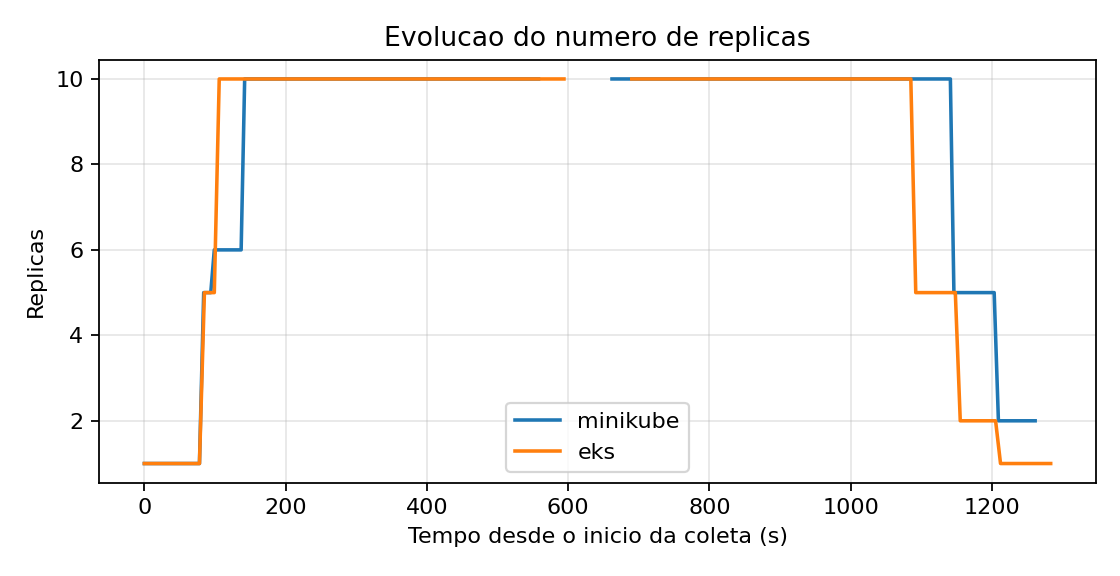
\includegraphics[width=0.92\textwidth]{figuras/replicas.png}
\caption{Evolução do número de réplicas nos dois ambientes}
\label{fig:replicas}
\end{figure}

\begin{figure}[ht]
\centering
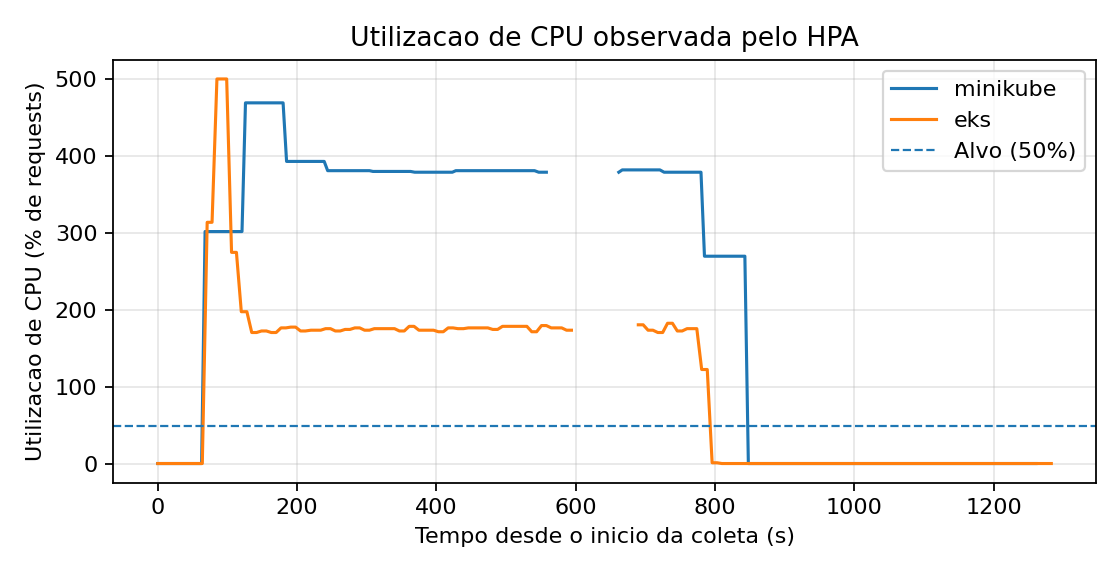
\includegraphics[width=0.92\textwidth]{figuras/cpu.png}
\caption{Utilização de processador observada pelo autoescalador}
\label{fig:cpu}
\end{figure}

\subsection{Latência de detecção}

O intervalo entre o início da carga e a criação da primeira réplica adicional
foi de 16 segundos no ambiente local e 14 segundos no gerenciado.

Esse resultado tem valor metodológico além do descritivo, pois indica que o
controlador se comporta de maneira equivalente nos dois ambientes. As
divergências observadas nas demais grandezas devem portanto ser atribuídas à
infraestrutura subjacente.

\subsection{Tempo até o teto de réplicas}

A diferença mais expressiva está no tempo necessário para sair de uma réplica e
atingir dez, de 74 segundos no ambiente local contra 35 segundos no gerenciado.

A diferença não decorre da decisão do controlador, e
sim da velocidade com que cada ambiente materializa réplicas. Duas causas são
plausíveis. O ambiente gerenciado utiliza \emph{containerd} diretamente,
enquanto o local interpõe o daemon Docker na criação de contêineres. Além disso,
o armazenamento do nó gerenciado é um volume dedicado, ao passo que o nó local
compartilha o disco da estação de trabalho com o sistema operacional e demais
processos.

Testes de autoescalamento conduzidos em
ambiente local tendem a subestimar a velocidade de resposta obtida em produção,
o que é conservador do ponto de vista de dimensionamento, porém pode induzir
ajustes desnecessários nas políticas.

\subsection{Comportamento no pico}

Em ambos os ambientes a utilização permaneceu substancialmente acima do alvo de
50 por cento mesmo com dez réplicas ativas. O controlador não conseguiu conduzir
a métrica ao valor desejado porque atingiu o limite superior configurado. Nesse
regime o autoescalador deixa de exercer controle e o sistema opera saturado.

O resultado evidencia que o teto de réplicas é decisão de capacidade e não
parâmetro formal. Um valor mal dimensionado transforma o mecanismo de
elasticidade em limitador de disponibilidade.

Nenhum Pod permaneceu em estado pendente em qualquer dos ambientes, o que
confirma que a capacidade dos nós foi suficiente para acomodar o teto de
réplicas e que as medidas de tempo refletem o comportamento do controlador e não
escassez de recursos.

\subsection{Redução}

O intervalo entre o fim da carga e o início da redução foi de 303 segundos nos
dois ambientes, contra os 300 segundos declarados na janela de estabilização.

A redução leva aproximadamente
vinte vezes mais tempo para iniciar do que o aumento, assimetria que decorre
diretamente das políticas configuradas e que corresponde ao comportamento
recomendado para ambientes de produção.

\section{Discussão}

\subsection{Custos}

Os dois ambientes possuem estruturas de custo qualitativamente distintas. O
ambiente local não apresenta custo marginal, pois utiliza equipamento já
disponível, e seu custo real manifesta-se como consumo de recursos da estação de
trabalho durante a execução.

O ambiente gerenciado apresenta três componentes cobrados por permanência,
independentemente de haver carga. O plano de controle é cobrado por hora desde
a criação do cluster, e permaneceu ativo por período considerável antes que
qualquer aplicação fosse implantada, em razão do tempo de provisionamento. A
instância do grupo de nós é cobrada enquanto existir. O volume de armazenamento
associado à instância segue a mesma lógica.

Cabe registrar que a distinção decisiva não está no valor absoluto, e sim no
regime de cobrança. O custo do ambiente gerenciado independe da existência de
carga, ao passo que a elasticidade que se buscou demonstrar atua apenas sobre a
camada de aplicação. Escalar Pods não reduz o custo do plano de controle nem do
nó provisionado.

\subsection{Facilidade de gerenciamento}

O ambiente local exigiu dois comandos para estar operacional, um para criar o
cluster e outro para habilitar o servidor de métricas. O ambiente gerenciado
exigiu a criação prévia de duas identidades no serviço de gerenciamento de
acesso, de uma rede virtual com três sub-redes por meio de pilha declarativa, do
cluster propriamente dito, de um grupo de nós, e a aplicação manual do manifesto
do servidor de métricas.

Essa assimetria não caracteriza deficiência do ambiente gerenciado. As
identidades e a rede existem porque o cluster opera em infraestrutura
compartilhada e multiusuário, na qual permissões e isolamento precisam ser
declarados. O ambiente local dispensa essas camadas porque não as possui.

A diferença mais instrutiva refere-se ao servidor de métricas. No ambiente local
trata-se de complemento habilitável por comando único, mantido pela própria
ferramenta. No ambiente gerenciado é responsabilidade do operador obter o
manifesto do projeto, escolher a versão e mantê-la atualizada. O provedor assume
o plano de controle, e não os componentes complementares executados sobre ele.

\subsection{Limitações}

A carga efetiva não foi rigorosamente idêntica nos dois ambientes. O gerador foi
configurado com paralelismo fixo de doze laços, e não com taxa de requisições
por segundo controlada. Como o ambiente local dispunha de maior capacidade de
processamento, o gerador emitiu mais requisições por unidade de tempo do que no
ambiente gerenciado. A consequência aparece nos valores de utilização observados
durante a fase de redução, de 382 por cento no ambiente local contra 183 por
cento no gerenciado.

As medidas de tempo permanecem válidas, uma vez que em ambos os casos a carga
excedeu amplamente o alvo e conduziu o sistema ao teto de réplicas. As medidas
de utilização absoluta, contudo, não são diretamente comparáveis entre os
ambientes. Um ensaio adicional com carga calibrada por taxa de requisições
permitiria comparação também nessa dimensão.

Os valores relatados decorrem de execução única por ambiente e não caracterizam
distribuição estatística. Repetições permitiriam estimar variabilidade e
distinguir diferenças sistemáticas de flutuações. Registre-se ainda que os picos
instantâneos de utilização mostraram-se ruidosos, tendo o ambiente gerenciado
apresentado pico superior na fase de subida e inferior na fase de redução, o que
reforça que a média em regime é a grandeza confiável.

Por fim, os nós dos dois ambientes possuem capacidades diferentes, de quatro e
dois processadores virtuais. O dimensionamento foi escolhido para que ambos
acomodassem o teto de dez réplicas sem Pods pendentes, condição verificada nos
resultados, porém a folga disponível não era equivalente.

\section{Conclusão}

O trabalho implantou o mesmo servidor web em cluster local e em cluster
gerenciado, submeteu ambos ao mesmo perfil de carga e mediu o comportamento do
autoescalador horizontal de Pods por meio de série temporal instrumentada.

Três conclusões decorrem dos resultados. A latência de detecção do controlador é
equivalente nos dois ambientes, próxima de um ciclo de reconciliação, o que
indica que o mecanismo de decisão independe da infraestrutura. O tempo
necessário para materializar as réplicas decididas difere por fator próximo de
dois, favorável ao ambiente gerenciado, e é atribuível ao \emph{runtime} de
contêineres e ao subsistema de armazenamento. A janela de estabilização de
redução foi reproduzida com desvio de 1 por cento nos dois ambientes, o que
valida a instrumentação empregada.

Do ponto de vista prático, o ambiente local mostrou-se adequado para validar a
correção da configuração, incluindo a presença de reservas de processador, a
disponibilidade do servidor de métricas e o comportamento das políticas
declaradas. Não se mostrou adequado para estimar tempos absolutos de resposta,
que foram sistematicamente superiores aos do ambiente gerenciado.

Como continuidade, três direções se apresentam. A calibração da carga por taxa
de requisições permitiria comparar também a utilização absoluta. A repetição dos
ensaios permitiria caracterizar variabilidade. A combinação do autoescalamento
de Pods com o autoescalamento de nós permitiria observar o comportamento quando
a capacidade do cluster deixa de ser suficiente, situação deliberadamente
evitada neste trabalho e que constitui limite natural do mecanismo estudado.

\section*{Disponibilidade}

O código da aplicação, os manifestos comentados, os scripts de instrumentação e
análise, as séries temporais coletadas e as evidências de execução estão
disponíveis em repositório público.

\begin{thebibliography}{9}

\bibitem{k8shpa}
Kubernetes Documentation.
\emph{Horizontal Pod Autoscaler Walkthrough}.
Disponível em
\url{https://kubernetes.io/docs/tasks/run-application/horizontal-pod-autoscale-walkthrough/}.

\bibitem{ekshpa}
Amazon Web Services.
\emph{Scale pod deployments with Horizontal Pod Autoscaler}.
AWS EKS User Guide. Disponível em
\url{https://docs.aws.amazon.com/eks/latest/userguide/horizontal-pod-autoscaler.html}.

\bibitem{k8sautoscaling}
Kubernetes Documentation.
\emph{Horizontal Pod Autoscaling}.
Disponível em
\url{https://kubernetes.io/docs/tasks/run-application/horizontal-pod-autoscale/}.

\bibitem{metricsserver}
Kubernetes SIGs.
\emph{Kubernetes Metrics Server}.
Disponível em \url{https://github.com/kubernetes-sigs/metrics-server}.

\bibitem{minikube}
Kubernetes Documentation.
\emph{minikube start}.
Disponível em \url{https://minikube.sigs.k8s.io/docs/start/}.

\end{thebibliography}

\end{document}
